\section{Energie- und Elektrizitätswirtschaft}

\subsection{Masseinheiten}

\begin{tabular}{|l|c|l|}
    \hline
    \textbf{Masseinheit}    & \textbf{Zeichen}  & \textbf{Umrechnung} \\
    \hline
    Watt                    & (W)               & \\ 
    Pferdestärke            & (PS)              & 1 PS $\approx$ 735 W \\ 
    \hline
    Joule                   & (J)               & \\ 
    Wattsekunde             & (Ws)              & 1 Ws = 1 J \\ 
    Kilowattstunde          & (kWh)             & 1 kWh = 3 600 000 J = 3,6 MJ \\ 
    Kalorie                 & (cal)             & 1 cal$_{IT}$ = 4,1868 J \\ 
    \hline
\end{tabular}


\subsection{Umrechnungsfaktoren}

\begin{tabular}{|l|c|c|c|c|}
    \hline
    \textbf{\textbf{Von | Zu}}  & \textbf{J = Ws}           & \textbf{kWh}                  & \textbf{GWh}              & \textbf{cal} \\
    \hline
            J = Ws              & 1                         & $0,2778 \cdot 10^{-6}$        & $0,2778 \cdot 10^{-12}$   & 0,2388 \\
            TJ                  & $1 \cdot 10^{12}$         & $0,2778 \cdot 10^{6}$         & 0,2778                    & $0,2388 \cdot 10^{12}$ \\
            kWh                 & $3,6 \cdot 10^{6}$        & 1                             & $1 \cdot 10^{-6}$         & $0,8598 \cdot 10^{6}$ \\
            GWh                 & $3,6 \cdot 10^{12}$       & $1 \cdot 10^{6}$              & 1                         & $0,8598 \cdot 10^{12}$ \\
            cal                 & 4,1868                    & $1,163 \cdot 10^{-6}$         & $1,163 \cdot 10^{-12}$    & 1 \\
    \hline
\end{tabular}


\subsection{Dezimalfaktoren}
\begin{tabular}{|l|c|r|}
    \hline
    \textbf{Bezeichnung}    & \textbf{Faktor}   & \textbf{Wert} \\
    \hline
    Kilo  (k)               & \(10^3\)          & 1 000 \\
    Mega  (M)               & \(10^6\)          & 1 000 000 \\
    Giga  (G)               & \(10^9\)          & 1 000 000 000 \\
    Tera  (T)               & \(10^{12}\)       & 1 000 000 000 000 \\
    Peta  (P)               & \(10^{15}\)       & 1 000 000 000 000 000 \\
    \hline
\end{tabular}


\subsection{Energien}

\subsubsection{Potentielle Energie $W_{\text{pot}}$}
$\boxed{W_{\text{pot}} = m \cdot g \cdot h}$ \quad $g = 9.81 \frac{m}{s^2}$

\renewcommand{\arraystretch}{1.2} % Erhöht Zeilenhöhe für bessere Lesbarkeit
\begin{tabular}{@{} l p {4cm} l @{}}
    $[W_{\text{pot}}]$  & Potentielle Energie   \dotfill & $Ws = Nm = J$ \\
    $[m]$               & Masse                 \dotfill & $kg$ \\
    $[g]$               & Erdbeschleunigung     \dotfill & $\frac{m}{s^2}$ \\
    $[h]$               & Höhenunterschied      \dotfill & $m$ \\
\end{tabular}

\subsubsection{Kinetsche Energie $W_{\text{kin}}$}
$\boxed{W_{\text{kin}} = \frac{1}{2} \cdot m \cdot v^2}$

\renewcommand{\arraystretch}{1.2} % Erhöht Zeilenhöhe für bessere Lesbarkeit
\begin{tabular}{@{} l p {4cm} l @{}}
    $[W_{\text{kin}}]$  & Kinetische Energie   \dotfill & $Ws = Nm = J$ \\
    $[m]$               & Masse                \dotfill & $kg$ \\
    $[v]$               & Geschwindigkeit      \dotfill & $m/s$ \\
\end{tabular}


\subsubsection{Feder Energie $W_{\text{F}}$}
$\boxed{W_{\text{F}} = \frac{1}{2} \cdot F \cdot s}$

\renewcommand{\arraystretch}{1.2} % Erhöht Zeilenhöhe für bessere Lesbarkeit
\begin{tabular}{@{} l p {4cm} l @{}}
    $[W_{\text{F}}]$  & Federenergie                \dotfill & $Ws = Nm = J$ \\
    $[F]$             & Kraft                       \dotfill & $N = kg \cdot m/s^2$ \\
    $[s]$             & Verschiebung (Auslenkung)   \dotfill & $m$ \\
\end{tabular}


\subsubsection{Kondensator Energie $W_{\text{C}}$}
$\boxed{W_{\text{C}} = \frac{1}{2} \cdot C \cdot U^2}$

\renewcommand{\arraystretch}{1.2} % Erhöht Zeilenhöhe für bessere Lesbarkeit
\begin{tabular}{@{} l p {4cm} l @{}}
    $[W_{\text{C}}]$  & Kondensatorenergie    \dotfill & $Ws = Nm = J$ \\
    $[C]$             & Kapazität             \dotfill & $F = \frac{As}{V}$ \\
    $[U]$             & Spannung              \dotfill & $V$ \\
\end{tabular}


\subsubsection{Induktivität Energie $W_{\text{L}}$}
$\boxed{W_{\text{L}} = \frac{1}{2} \cdot L \cdot I^2}$

\renewcommand{\arraystretch}{1.2} % Erhöht Zeilenhöhe für bessere Lesbarkeit
\begin{tabular}{@{} l p {4cm} l @{}}
    $[W_{\text{L}}]$  & Induktivitätsenergie  \dotfill & $Ws = Nm = J$ \\
    $[L]$             & Induktivität          \dotfill & $H = \frac{Vs}{A}$ \\
    $[I]$             & Stromstärke           \dotfill & $A$ \\
\end{tabular}


\subsubsection{Batterie Energie $W_{\text{bat}}$}
$\boxed{W_{\text{bat}} = Q \cdot U}$

\renewcommand{\arraystretch}{1.2} % Erhöht Zeilenhöhe für bessere Lesbarkeit
\begin{tabular}{@{} l p {4cm} l @{}}
    $[W_{\text{bat}}]$  & Batterieenergie       \dotfill & $Ws = Nm = J$ \\
    $[Q]$               & Elektrische Ladung    \dotfill & $C = As$ \\
    $[U]$               & Spannung              \dotfill & $V$ \\
\end{tabular}


\subsubsection{Thermische Energie $W_{\text{th}}$}
$\boxed{W_{\text{th}} = m \cdot c \cdot (\vartheta_1 - \vartheta_2)}$ \quad $c_{Wasser} = 4187 \frac{J}{kg \cdot K}$

\renewcommand{\arraystretch}{1.2} % Erhöht Zeilenhöhe für bessere Lesbarkeit
\begin{tabular}{@{} l p {4cm} l @{}}
    $[W_{\text{th}}]$       & Thermische Energie          \dotfill & $Ws = Nm = J$ \\
    $[m]$                   & Masse                       \dotfill & $kg$ \\
    $[c]$                   & Spezifische Wärmekapazität  \dotfill & $\frac{J}{kg \cdot K}$ \\
    $[\vartheta_1]$         & Anfangstemperatur           \dotfill & $^\circ C$ oder $K$ \\
    $[\vartheta_2]$         & Endtemperatur               \dotfill & $^\circ C$ oder $K$ \\
\end{tabular}



\subsubsection{Spezifische Energie $e$}

$\boxed{e = \frac{W}{m}}$ \quad $\boxed{W = e \cdot m}$

\renewcommand{\arraystretch}{1.2} % Erhöht Zeilenhöhe für bessere Lesbarkeit
\begin{tabular}{@{} l p {4cm} l @{}}
    $[e]$  & Spezifische Energie    \dotfill & $\frac{J}{kg}$ \\
    $[W]$  & Gesamtenergie          \dotfill & $J$ \\
    $[m]$  & Masse                  \dotfill & $kg$ \\
\end{tabular}


\subsubsection{Rotations Energie $W_{\text{rot}}$}
$\boxed{W_{\text{rot}} = \frac{1}{2} \cdot J \cdot \omega^2 }$ \quad $\boxed{W_{\text{rot}} = 2 \cdot J \cdot \pi^2 \cdot f^2 }$ \quad $\boxed{W_{\text{rot}} = \frac{J \cdot \pi^2 \cdot n^2}{1800}}$

$\boxed{\omega = 2 \cdot \pi \cdot f}$ \quad $\boxed{f = \frac{n}{60}}$ \quad $\boxed{n = f \cdot 60}$


\renewcommand{\arraystretch}{1.2} % Erhöht Zeilenhöhe für bessere Lesbarkeit
\begin{tabular}{@{} l p {5cm} l @{}}
    $[W_{\text{rot}}]$  & Rotationsenergie                      \dotfill & $Ws = Nm = J$ \\
    $[J]$               & Trägheitsmoment                       \dotfill & $kg \cdot m^2$ \\
    $[\omega]$          & Winkelgeschwindigkeit                 \dotfill & $\frac{rad}{s}$ \\
    $[f]$               & Drehfrequenz, Umdrehungen pro Sekunde \dotfill & $\frac{1}{s} = \frac{U}{\text{sek}}$ \\
    $[n]$               & Umdrehungen pro Minute                \dotfill & $\frac{1}{\text{min}} = \frac{U}{\text{min}}$ \\
\end{tabular}

\vspace{0.25cm}
\myul{\textbf{Massenträgheitsmoment $J$}}\\
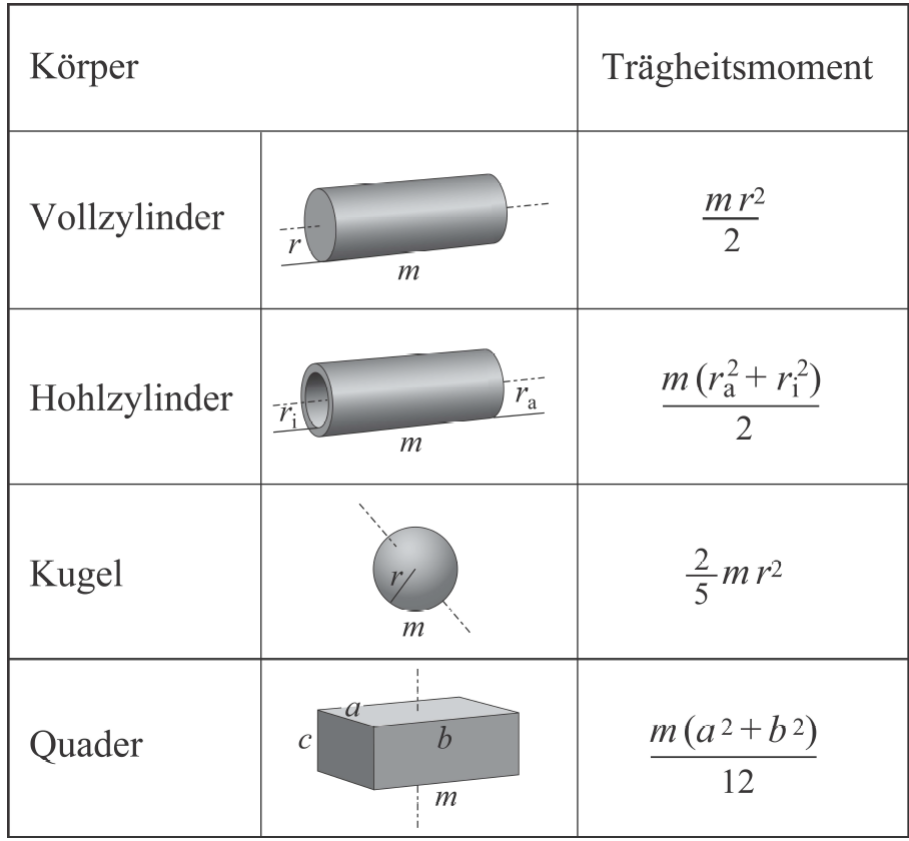
\includegraphics[width=0.75\linewidth]{images/Physik_1-Mechanik.png}


\subsection{Leistung}

\subsubsection{Rotations Leistung $P_{rot}$}
$\boxed{P = M \cdot \omega}$ \quad $\boxed{P = M \cdot 2 \cdot \pi \cdot f }$ \quad $\boxed{P = \frac{M \cdot 2 \cdot \pi \cdot n}{60} }$

\renewcommand{\arraystretch}{1.2} % Erhöht Zeilenhöhe für bessere Lesbarkeit
\begin{tabular}{@{} l p {4cm} l @{}}
    $[P_{rot}]$ & Rotations Leistung        \dotfill & $W = \frac{J}{s} = \frac{Nm}{s}$ \\
    $[M]$       & Drehmoment                \dotfill & $Nm$ \\
    $[\omega]$  & Winkelgeschwindigkeit     \dotfill & $\frac{rad}{s}$ \\
    $[f]$       & Drehfrequenz              \dotfill & $Hz = \frac{1}{s}$ \\
    $[n]$       & Umdrehungen pro Minute    \dotfill & $\frac{1}{\text{min}} = \frac{U}{\text{min}}$ \\
\end{tabular}


\subsubsection{Thermische Leistung $P_{\text{th}}$}
$\boxed{P_{\text{th}} = \dot{m} \cdot c \cdot \Delta \vartheta}$ \quad $\boxed{\dot{m} = \rho \cdot \dot{V} }$

\renewcommand{\arraystretch}{1.2} % Erhöht Zeilenhöhe für bessere Lesbarkeit
\begin{tabular}{@{} l p {4cm} l @{}}
    $[P_{\text{th}}]$       & Thermische Leistung           \dotfill & $W = \frac{J}{s}$ \\
    $[\dot{m}]$             & Massenstrom                   \dotfill & $\frac{kg}{s}$ \\
    $[c]$                   & Spezifische Wärmekapazität    \dotfill & $\frac{J}{kg \cdot K}$ \\
    $[\Delta \vartheta]$    & Temperaturdifferenz           \dotfill & $K$ oder $^\circ C$ \\
    $[\rho]$                & Dichte                        \dotfill & $\frac{kg}{m^3}$ \\
    $[\dot{V}]$             & Volumenstrom                  \dotfill & $\frac{m^3}{s}$ \\
\end{tabular}


\subsubsection{Transmissions Wärmeverlustleistung $P_{VW}$}

$\boxed{P_{VW} = U \cdot A \cdot \Delta \vartheta}$

\renewcommand{\arraystretch}{1.2} % Erhöht Zeilenhöhe für bessere Lesbarkeit
\begin{tabular}{@{} l p {4cm} l @{}}
    $[P_{VW}]$              & Wärmeverlustleistung          \dotfill & $W = \frac{J}{s}$ \\
    $[U]$                   & Wärmedurchgangskoeffizient    \dotfill & $\frac{W}{m^2 \cdot K}$ \\
    $[A]$                   & Fläche                        \dotfill & $m^2$ \\
    $[\Delta \vartheta]$    & Temperaturdifferenz           \dotfill & $K$ \\
\end{tabular}


\subsubsection{Mechanische Leistung $P_{v}$}
$\boxed{P_v = F \cdot v}$ \quad $\boxed{F = m \cdot g}$

\renewcommand{\arraystretch}{1.2} % Erhöht Zeilenhöhe für bessere Lesbarkeit
\begin{tabular}{@{} l p {4cm} l @{}}
    $[P_v]$ & Mechanische Leistung   \dotfill & $W = \frac{J}{s} = Nm/s$ \\
    $[F]$   & Kraft                  \dotfill & $N = kg \cdot \frac{m}{s^2}$ \\
    $[m]$   & Masse                  \dotfill & $kg$ \\
    $[g]$   & Erdbeschleunigung      \dotfill & $\frac{m}{s^2}$ \\
    $[v]$   & Geschwindigkeit        \dotfill & $\frac{m}{s}$ \\
\end{tabular}


\subsubsection{Leistung der Solaranlage $P_{PV}$}
$\boxed{P_{PV} = \eta \cdot A \cdot E}$

\renewcommand{\arraystretch}{1.2} % Erhöht Zeilenhöhe für bessere Lesbarkeit
\begin{tabular}{@{} l p {4cm} l @{}}
    $[P_{PV}]$      & Elektrische Leistung         \dotfill & $W = J/s$ \\
    $[\eta]$        & Wirkungsgrad                 \dotfill & $-$ \\
    $[A]$           & Fläche der Solaranlage       \dotfill & $m^2$ \\
    $[E]$           & Einstrahlung                 \dotfill & $\frac{W}{m^2}$ \\
\end{tabular}


\subsubsection{Leistung eines Wasserkraftwerks $P$}
$\boxed{P = \eta \cdot \rho \cdot g \cdot \dot{V} \cdot h}$

\renewcommand{\arraystretch}{1.2} % Erhöht Zeilenhöhe für bessere Lesbarkeit
\begin{tabular}{@{} l p {4cm} l @{}}
    $[P]$       & Elektrische Leistung          \dotfill & $W = J/s$ \\
    $[\eta]$    & Wirkungsgrad                  \dotfill & $-$ \\
    $[\rho]$    & Dichte                        \dotfill & $\frac{kg}{m^3}$ \\
    $[g]$       & Erdbeschleunigung             \dotfill & $\frac{m}{s^2}$ \\
    $[\dot{V}]$ & Volumenstrom                  \dotfill & $\frac{m^3}{s}$ \\
    $[h]$       & Höhendifferenz                \dotfill & $m$ \\
\end{tabular}


\subsubsection{Drehstrom Leistungsberechnung $P_{\circlearrowleft}$}
$\boxed{P_{\circlearrowleft} = \sqrt{3} \cdot U \cdot I \cdot \cos(\varphi)}$

\renewcommand{\arraystretch}{1.2} % Erhöht Zeilenhöhe für bessere Lesbarkeit
\begin{tabular}{@{} l p {4cm} l @{}}
    $[P_{\circlearrowleft}]$    & Wirkleistung              \dotfill & $W = J/s$ \\
    $[U]$                       & Verkettete Spannung       \dotfill & $V$ \\
    $[I]$                       & Stromstärke               \dotfill & $A$ \\
    $[\cos(\varphi)]$           & Leistungsfaktor   \dotfill & $-$ \\
\end{tabular}


\subsection{Schweizer Strom-Mix}
$
\begin{array}{|c|l|}
    \hline
    38.1 \% & \text{Kernkraft} \\ \hline
    32.3 \% & \text{Speicherkraftwerke} \\ \hline
    24.2 \% & \text{Laufkraftwerke} \\ \hline
    5.4 \% & \text{konventionell-thermische Kraftwerke} \\ \hline
\end{array}
$

$
\begin{tabular}{|c|l|}
    \hline
    1.52 \% & Kehrichtverbrennungsanlagen \\ \hline
    0.29 \% & Biomasse \\ \hline
    0.19 \% & Abwasserreinigungsanlagen \\ \hline
    0.13 \% & Photovoltaik \\ \hline
    0.06 \% & Windkraft \\ \hline
\end{tabular}
$


\newcolumn
\subsection{Investitions- und Kostenrechnung}

\subsubsection{Annuitätsfaktor $A$}
$\boxed{A = \frac{(1 + i)^n \cdot i}{(1 + i)^n - 1}}$

\renewcommand{\arraystretch}{1.2} % Erhöht Zeilenhöhe für bessere Lesbarkeit
\begin{tabular}{@{} l p {4cm} l @{}}
    $[A]$       & Annuitätsfaktor           \dotfill & $1$ \\
    $[i]$       & Zinsen                    \dotfill & $1$ \\
    $[n]$       & Anzahl Jahre Laufzeit     \dotfill & $1$ \\
\end{tabular}


\subsubsection{Kapitalkosten $K_{\text{K}}$}
$\boxed{K_{\text{K}} = A \cdot I}$

\renewcommand{\arraystretch}{1.2} % Erhöht Zeilenhöhe für bessere Lesbarkeit
\begin{tabular}{@{} l p {4cm} l @{}}
    $[K_{\text{K}}]$    & Kapitalkosten     \dotfill & CHF oder € \\
    $[A]$               & Annuitätsfaktor   \dotfill & $1$ \\
    $[I]$               & Investitionen     \dotfill & CHF oder € \\
\end{tabular}


\subsubsection{Unterhaltskosten $K_{\text{U}}$}
$\boxed{K_{\text{U}} = p_{\text{U}} \cdot I}$

\renewcommand{\arraystretch}{1.2} % Erhöht Zeilenhöhe für bessere Lesbarkeit
\begin{tabular}{@{} l p {4cm} l @{}}
    $[K_{\text{U}}]$    & Unterhaltskosten              \dotfill & CHF oder € \\
    $[p_{\text{U}}]$    & Unterhaltskosten-Prozentsatz  \dotfill & $1$ \\
    $[I]$               & Investitionen                 \dotfill & CHF oder € \\
\end{tabular}


\subsubsection{Fix-Kosten $K_{\text{Fix}}$}
$\boxed{K_{\text{Fix}} = K_{\text{K}} + K_{\text{U}} = (A + p_{\text{U}}) \cdot I}$

\renewcommand{\arraystretch}{1.2} % Erhöht Zeilenhöhe für bessere Lesbarkeit
\begin{tabular}{@{} l p {4cm} l @{}}
    $[K_{\text{Fix}}]$    & Fix-Kosten              \dotfill & CHF oder € \\
\end{tabular}


\subsubsection{Erlös oder Deckungsbeitrag $E$}
$\boxed{E = t_{\text{VL}} \cdot C \cdot P}$

\renewcommand{\arraystretch}{1.2} % Erhöht Zeilenhöhe für bessere Lesbarkeit
\begin{tabular}{@{} l p {4cm} l @{}}
    $[E]$               & Erlös             \dotfill & CHF oder € \\
    $[t_{\text{VL}}]$   & Volllaststunden   \dotfill & $h$ \\
    $[C]$               & Grenzkosten       \dotfill & $\frac{\text{CHF}}{\text{MWh}}$ oder $\frac{\text{€}}{\text{MWh}}$ \\
    $[P]$               & Leistung          \dotfill & $W = \frac{Nm}{s} = \frac{J}{s}$ \\
\end{tabular}


\subsubsection{Ergebnis (Gewinn oder Verlust) $G$}
$\boxed{G = E - K_{\text{Fix}} - K_{\text{Var}}}$

\subsubsection{Variable Kosten $K_{\text{V}}$}

\renewcommand{\arraystretch}{1.2} % Erhöht Zeilenhöhe für bessere Lesbarkeit
\begin{tabular}{@{} l p {4cm} l @{}}
    $[G]$               & Ergebnis        \dotfill & CHF oder € \\
    $[E]$               & Erlös           \dotfill & CHF oder € \\
    $[K_{\text{Fix}}]$  & Fix-Kosten      \dotfill & CHF oder € \\
    $[K_{\text{Var}}]$  & Variable Kosten \dotfill & CHF oder € \\
\end{tabular}







































